%! TEX root = 'main.tex'
\section{Background}
\label{sec:implant-background}

This section provides background knowledge for the rest of the paper. We first introduce the industrial control system (ICS) and a provide detailed information about the programmable logic controller (PLC). Then we provide detailed technical background on I2C and JTAG protocols, that is required for the paper.

\textbf{\texttt{ICS}} is a distributed system used for industrial process control. It connects sensors and actuators that interact with the physical systems (e.g., power grid) with the cyber components such as networks and servers. In a factory, local operations are often controlled by PLCs that receive supervisory commands from a remote host. For example, a human operator monitors the system's state and sends out instructions through a human-machine interface (HMI). Most PLCs and HMI hosts are connected to the ICS via Ethernet.

\textbf{\textit{PLC}}. PLCs are industrial grade computers designed to run over an extended period of time without restarting. They are rigorously tested to withstand operating in an industrial environment where they are exposed to vibration and noise. PLCs consist of a microcontroller, I/O modules, a power supply, and other specialized addon modules. The I/O modules of PLCs interact with the physical world, gathering digital inputs from sensors, switch, or a thermometer. The microcontroller serves as the PLC's brain, executing pre-programmed IEC 61131-3 languages programs such as ladder logic to give operating signals to the output modules based on the inputs. 

The PLCs usually uses a fix-interval timer to run compiled ladder logic repeatedly, which is the so-called scan cycle. Any changes to the I/O modules appear only at the end of scan cycle. PLC interacts with the IO module is through the GPIO ports on the microcontroller. Essentially, each digital input/output in the PLC has a corresponding GPIO bit. The PLC also has an LED panel that indicates each IO pin's status, which roughly gives an idea of whether the PLC is functioning correctly. The firmware of PLC either contains a real-time operating system or code that runs bare-metally on the microcontroller. The PLC usually provides library routines to operate on various I/O devices such as I2C, SPI~\cite{leens2009introduction} and CAN bus~\cite{bozdal2018survey}. However, the vendors do not shared these information with the users. In this paper, we extracted these libraries from ROM, which is discussed in  \autoref{sec:implant-design}.

\textbf{\textit{I2C}} is a serial protocol that connects low-speed devices such as EEPROM in embedded systems. The I2C bus only has two wires, namely, SCL and SDA (the third wire connects to the ground). SCL is the clock line that synchronizes all data transfers over the I2C bus, and the SDA is the data line. All the low-speed devices in the system can be connected to the same I2C bus as slave devices, where each device has a unique address. The master device initiates a transaction by sending a high-to-low signal on the SDA while keeps SCL high. It is called a start condition. After that, the master sends the target device address byte onto the bus. The first 7 bits are the address, and the last bit indicates the data direction where one indicates reading, zero indicates writing. Only the device that matches this address continues with this transaction. It acknowledges this byte by pulling SDA low during the next SCL pulse. After addressing the target device, the master sends out the target device's internal location or register number. Next, the master device sends the data. The target device automatically increases its internal register address after receiving each byte. When the transaction is complete, the master device sends a stop sequence onto the bus.


\textbf{\textit{JTAG}} is a IEEE1149.1 standard, which is used for testing printed circuit boards using boundary-scan. The JTAG interface uses very few pins (TDI, TDO, TMS, TCK, and TRST) to connect to an on-chip Test Access Port (TAP) that implements a stateful protocol, as shown in ~\autoref{fig:jtagsm}.  One or more devices can expose multiple TAPs in a daisy chain, also known as a scan chain. The host communicates with the TAPs by manipulating TMS and TDI in conjunction with TCK and reading results through TDO.

\textcolor{red}{should visit this part later}

\begin{figure}[ht]
	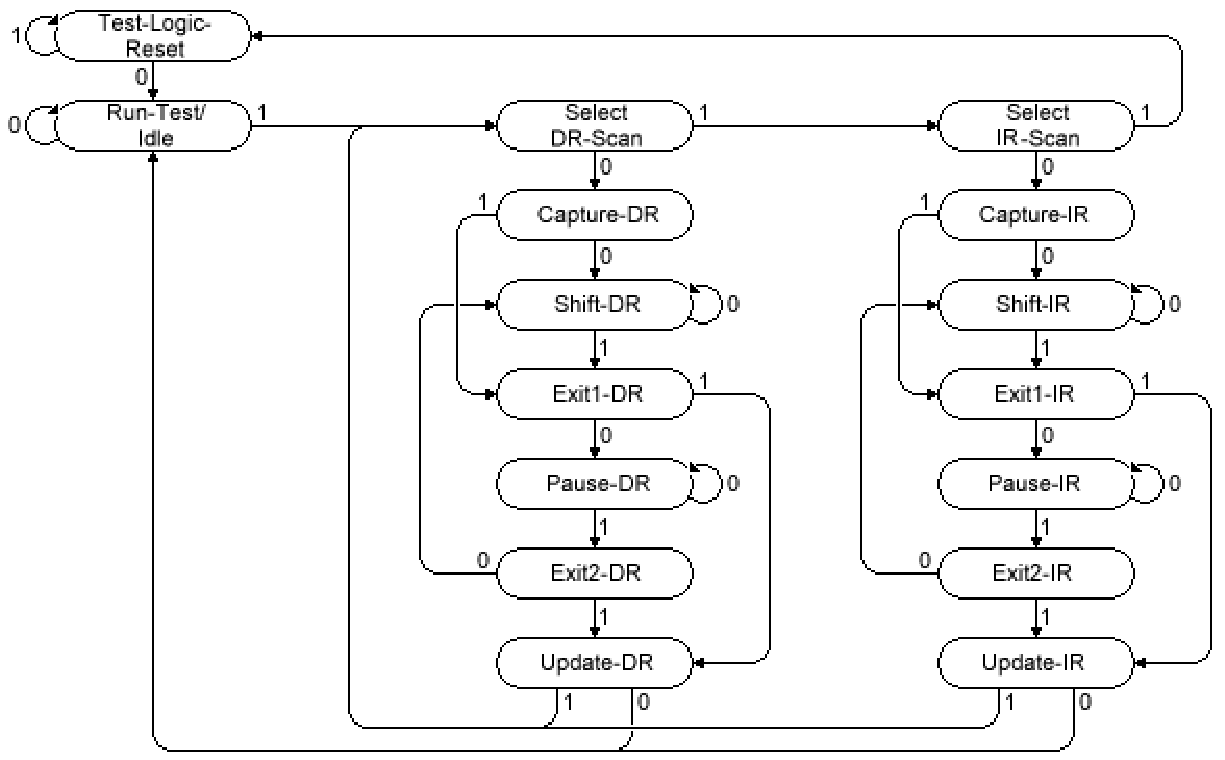
\includegraphics[width=0.47\textwidth]{figures/jtagsm}
	\centering
	\caption{JTAG TAP state machine.}
	\label{fig:jtagsm}
\end{figure}


The JTAG standard has four common registers: Instruction Register (IR) and Data Register (DR),  IDCODE, and BYPASS. The IDCODE register contains data that uses a standardized format that includes a manufacturer code. The BYPASS register is a single-bit data register that allows this device to be bypassed (do nothing) while other devices in the scan chain are examined. The IR and DR register's size depends on the TAP implementation, and they are used to send in instruction and receive result data.

The TAP implementation defines instructions and associated them with internal data registers. For instance, the host sends the IDCODE instruction through IR and subsequently gets the value of a 32-bit register (IDCODE) from TDO.

The PLC we used in this paper uses an ARM core microcontroller, namely, Texas Instruments Stellaris LM3S2793~\cite{lm3s2793}. The debug functionality provided in LM3S2793 is as CoreSight components. It provides real-time access for the debugger without halting the processor to AMBA (Advanced Microcontroller Bus Architecture)~\cite{flynn1997amba} system memory, peripheral registers, and all debug configuration registers. The TAP controller is implemented using CoreSight technologies, and it is called Debug Access Port (DAP) instead.

\begin{figure}[ht]
	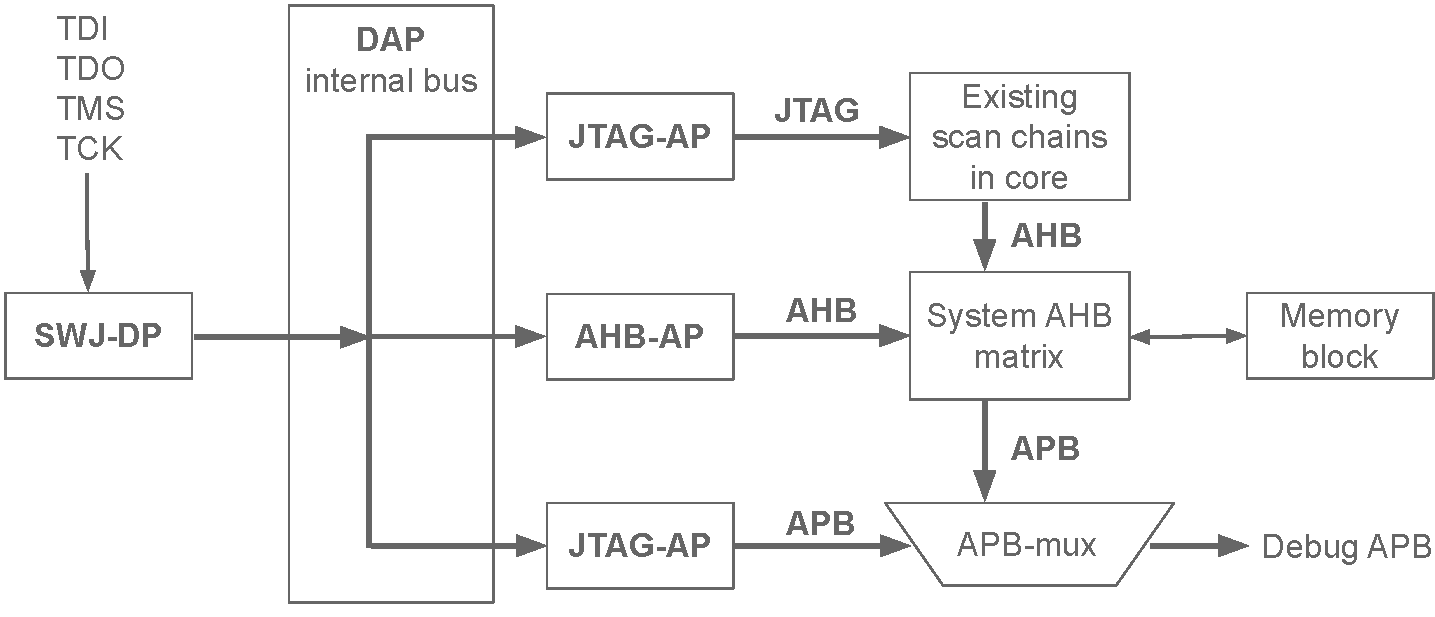
\includegraphics[width=0.47\textwidth]{figures/dap}
	\centering
	\caption{The debug port (DP) receives host signals and maintains the JTAG state machine. The instruction and data are sent to the DAP core through IR and DR, respectively. Unlike the JTAG standard that needs to halt the processor before reading registers, using CoreSight DAP, the registers, SARM, and MMIO can be accessed during runtime without halting the processor.}
	\label{fig:dap}
\end{figure}


As shown in~\autoref{fig:dap}, each DAP contains Debug Ports (DPs) and Access Ports (APs). The DP provides access to the DAP from an external debugger. Then the DAP uses the APs to access on-chip resources. Multiple APs such as AHP-AP, ABP-AP, and JTAG-AP respond to each type of bus and the devices that connect to it. For instance, the AHB-AP provides an AHB-Lite master for accessing the system AHB bus, which we use to access the RAM and MMIO.



